% !TeX spellcheck = en_GB
% !TeX program = lualatex
%
% v 2.3  Feb 2019   Volker RW Schaa
%		# changes in the collaboration therefore updated file "jacow-collaboration.tex"
%		# all References with DOIs have their period/full stop before the DOI (after pp. or year)
%		# in the author/affiliation block all ZIP codes in square brackets removed as it was not %         understood as optional parameter and ZIP codes had bin put in brackets
%       # References to the current IPAC are changed to "IPAC'19, Melbourne, Australia"
%       # font for ‘url’ style changed to ‘newtxtt’ as it is easier to distinguish "O" and "0"
%
\documentclass
[
    a4paper,
    %boxit,        % check whether paper is inside correct margins
    %titlepage,    % separate title page
    %refpage       % separate references
    % biblatex,     % biblatex is used
    %keeplastbox,   % flushend option: not to un-indent last line in References
    nospread,     % flushend option: do not fill with whitespace to balance columns
    %hyphens,      % allow \url to hyphenate at "-" (hyphens)
    %xetex,        % use XeLaTeX to process the file
    %luatex,       % use LuaLaTeX to process the file
]{jacow}
%
% ONLY FOR \footnote in table/tabular
%
\usepackage{pdfpages,multirow,ragged2e} %

%
% To define glossaries
%
\usepackage[acronym]{glossaries}

%
% if BibLaTeX is used
%
\ifboolexpr{bool{jacowbiblatex}}%
 {%
  \addbibresource{references.bib}
 }{}
\listfiles

%
% New commands
%
\newcommand*{\rom}[1]{\uppercase\expandafter{\romannumeral#1\relax}}
\providecommand{\der}{\mathrm{d}}
\providecommand{\rf}{\mathrm{rf}}
\providecommand{\Real}[1]{\ensuremath{\mathrm{Re}\left\{#1\right\}}}

%
% Glossaries
%
\newacronym{3hc}{3HC}{third-harmonic cavity}
\newacronym{dcct}{DCCT}{direct-current current transformer}
\newacronym{dft}{DFT}{discrete Fourier transform}
\newglossaryentry{bbb}
{
    name={BbB},
    description={bunch-by-bunch feedback system},
    first={bunch-by-bunch (\glsentrytext{bbb}) feedback system},
}
\newglossaryentry{hom}
{
    name={HOM},
    description={higher-order mode},
    first={higher-order mode (\glsentrytext{hom})},
    plural={HOMs},
    descriptionplural={higher-order modes},
    firstplural={higher-order modes (\glsentryplural{hom})}
}


\begin{document}
\title{Broadband impedance induced heating proxy for operation at higher total current at SIRIUS}
\author
{
    F. H. de Sá\thanks{murilo.alves@lnls.br}\textsuperscript{1},
    I. C. de Almeida\textsuperscript{1},
    M. B. Alves\textsuperscript{1,2},
    G. Gomes\textsuperscript{3},
    L. Liu\textsuperscript{1},
    X. Resende\textsuperscript{1}\\
    \textsuperscript{1}Brazilian Synchrotron Light Laboratory -- LNLS, Campinas, Brazil\\
    \textsuperscript{2}Gleb Wataghin Institute of Physics, University of Campinas -- UNICAMP, Campinas, Brazil\\
    \textsuperscript{3}Brazilian Center for Research in Energy and Materials -- CNPEM, Campinas, Brazil
}
\maketitle

\begin{abstract}
    SIRIUS, a brazilian~4\textsuperscript{th}~generation synchrotron light source, currently operates in top-up mode at~\SI{100}{\milli\ampere} in uniform fill. The main limiting factor for reaching higher currents is the temporary RF system in use. It is comprised of one PETRA 7-Cell cavity and two solid state amplifier towers that combined provide at most~\SI{120}{\kilo\watt} of power. By mid~\num{2024}, two superconducting RF cavities will replace the current cavity and two amplifier towers will be added to the system, allowing operation at higher currents. The design current of SIRIUS storage ring is~\SI{350}{\milli\ampere}, which can only be achieved once a third harmonic cavity is installed to lengthen the bunches to avoid excessive wake-induced heating of sensitive components. However, the installation of such cavity is not foreseen in the near future, which raises the question of which is the maximum current in uniform fill SIRIUS can be operated. This work will present some theoretical and experimental studies carried out to answer this question.
\end{abstract} 

\section{Introduction}
    SIRIUS RF power plant upgrade will be ready for commissioning in October of 2024. Once this system is operating, it will allow increasing the stored current in users operations to~\SI{350}{\milli\ampere} with the design nominal voltage of~\SI{3}{\mega\volt}, considering the energy loss by dipoles and all the undulators of Phase~\rom{1} of operation. The expected natural bunch length at this voltage is approximately~\SI{2.4}{\milli\meter}. This short bunch imposes a large wake-field induced heat-load on the accelerator components and shorten the Touschek lifetime. A~\gls{3hc} is considered to lengthen the bunches and alleviate these effects, but its installation is not planned for the near future. For this reason, it is important to estimate the maximum stored current SIRIUS storage ring can operate without the~\gls{3hc}.

    One way to estimate the heating load for higher currents involves using different filling patterns. According to the the impedance budget model, most of the heating load of SIRIUS storage ring is due to broadband impedances. For this type of wake-field, the heat-load depends on the squared sum of the filling pattern vector and on the total current squared. This fact is useful for estimation of the heat load for SIRIUS because the current total power available by the RF system limits the maximum stored current to~\SI{100}{\milli\ampere}, with a gap voltage of~\SI{\sim1.6}{\mega\volt}. SIRIUS operates with uniform filling, which has the smallest possible squared sum. In this way, by using any other filling patterns at~\SI{100}{\milli\ampere}, we can estimate the heating load of the uniform filling at higher currents.

    Given the limited RF power, another way of estimating the heat-load for future operations consists in increasing the total stored current with a lower gap voltage to reduce the power consumption of the cavity. Currently, SIRIUS operates with a PETRA 7-Cell cavity at a gap voltage of~\SI{\sim1.6}{\mega\volt} with a total power of~\SI{\sim100}{\kilo\watt}. From this,~\SI{\sim50}{\kilo\watt} is used to keep the gap voltage and the remaining power is consumed by the~\SI{100}{\milli\ampere} beam. Decreasing the gap voltage to~\SI{\sim0.7}{\mega\volt} would still keep the Touschek lifetime above~\SI{1}{\hour} (the energy loss per turn in SIRIUS storage ring is~\SI{\sim480}{\kilo\electronvolt}) and allow a maximum stored current of~\SI{\sim170}{\milli\ampere}. This method has the advantage of keeping the same filling pattern of regular operation, thus sampling the impedance at the same harmonics, which also serves as an estimate of the effect of narrow band impedance sources. On the other hand, the bunch length is longer at lower gap voltages, which limits the frequency range of the impedance sampled by the beam and underestimate the broadband effect. 

    This work will describe the experimental and theoretical studies carried out to estimate the maximum beam current SIRIUS can operate, while keeping a reasonable lifetime for top-up operation and no heating issues, using both approaches described above.

\section{Theory of Heating Load}
    The power deposited by the beam in a component of the vacuum chamber is given by~\cite{Chao:1993zn}:
    \begin{equation}\label{eq:power_general}
        P = I_\mathrm{t}^2T_0 \frac{\omega_0}{2\pi}\sum_{p=-\infty}^{\infty} \left|\tilde{\lambda}(p\omega_0)\right|^2\Real{Z(p\omega_0)},
    \end{equation}
    where $I_\mathrm{t}>0$ is the total current of the beam, $T_0$ and $\omega_0$ are the revolution period and angular frequency of the storage ring, $Z$ is the longitudinal impedance of the component and 
    \begin{equation}
        \tilde{\lambda}(\omega) = \int_{-\infty}^\infty\der z \lambda(z) e^{i\omega z/c},
    \end{equation}
    where $c$ is the speed of light and $\lambda(z)$ is the longitudinal distribution of the beam, which can be written as
    $
        \lambda(z) = \sum_{\ell=0}^{h-1} F_\ell \lambda_\ell(z - \ell \lambda_\rf)
    $,
    where $h$ is the harmonic number of the ring, $\lambda_\rf=cT_0/h$ is the rf wavelength, $\lambda_\ell(z)$ is the distribution of the $\ell$-th bunch and $F_\ell \ge 0$ are the components of the filling pattern vector,
    $
    F = \left(\frac{I_0}{I_\mathrm{t}},\dots, \frac{I_{h-1}}{I_\mathrm{t}}\right)^\mathrm{T}
    $,
    which has unit sum. Since the bunch distributions are normalized to unity, so is the beam distribution.
    
    The Fourier transform of the longitudinal distribution is then given by
    $
        \tilde{\lambda}(\omega) = \sum_{\ell=0}^{h-1}F_\ell\tilde{\lambda_\ell}(\omega)e^{i\ell\omega \lambda_\rf/c}
    $
    and its squared modulus is
    \begin{equation}\label{eq:modulus_squared}
        \left|\tilde{\lambda}(\omega)\right|^2 = \left|\tilde{\lambda_0}(\omega)\right|^2 \left|B(\omega)\right|^2,
    \end{equation}
    where we defined the quantity $B(\omega) = \sum_{\ell=0}^{h-1}F_\ell e^{i\ell\omega \lambda_\rf/c}$
    and assumed all bunch distributions are equal to $\lambda_0(z)$.

    Inserting Eq.~\eqref{eq:modulus_squared} in Eq.~\eqref{eq:power_general}, we get
    \begin{equation}
        P = I_\mathrm{t}^2T_0 \frac{\omega_0}{2\pi}\sum_{p=-\infty}^{\infty} \left|\tilde{\lambda_0}(\omega_p)\right|^2 \left|B(\omega_p)\right|^2\Real{Z(\omega_p)},
    \end{equation}
    where $\omega_p = p\omega_0$. Note that
    $
        B(\omega_p) = \sum_{\ell=0}^{h-1}F_\ell e^{i2\pi p\ell/h} = \mathrm{DFT}(F)^*_p,
    $
    where $\mathrm{DFT}(F)^*_p$ denotes the complex conjugate of the $p$-th component of the \gls{dft} of the filling pattern vector. Since the filling pattern has length $h$, its \gls{dft} has the property:
    $
        B((p+h)\omega_0) = B(p\omega_0)
    $,
    which allows us to write the power loss in the following convenient form
    \begin{equation}
        P = I_\mathrm{t}^2T_0 \frac{\omega_0}{2\pi}\sum_{\ell=0}^{h-1} \left|B(\ell\omega_0)\right|^2\sum_{p=-\infty}^{\infty} \left|\tilde{\lambda_0}(\omega_{pl})\right|^2 \Real{Z(\omega_{pl})},
    \end{equation}
    where $\omega_{pl} = (ph+\ell)\omega_0$.
    
    Now, we assume the impedance varies slowly in the frequency scale of the rf frequency, i.e., it is a broadband impedance,
    $
        Z((ph+\ell)\omega_0) \approx Z(ph\omega_0), \, \forall\, p \in\mathbb{Z}\,\,\mathrm{and}\,\, \ell \in[0,h-1],
    $
    and that the distribution also varies slowly. Using Parseval's theorem for the~\gls{dft}~\cite{Wikipedia_DFT},
    $
        \sum_{\ell=0}^{h-1} \left|B(\ell\omega_0)\right|^2 = h\sum_{\ell=0}^{h-1} F_\ell^2 = h|F|^2,
    $
    we can write the power loss as
    \begin{equation}
        P \approx I_\mathrm{t}^2 \left|F\right|^2 T_0 \frac{h\omega_0}{2\pi}\sum_{p=-\infty}^{\infty} \left|\tilde{\lambda_0}(\bar{\omega}_p)\right|^2 \Real{Z(\bar{\omega}_p)},
    \end{equation}
    where $\bar{\omega}_p = ph\omega_0$. Defining the loss factor
    $
        \kappa = \frac{h\omega_0}{2\pi}\sum_{p=-\infty}^{\infty} \left|\tilde{\lambda_0}(\bar{\omega}_p)\right|^2 \Real{Z(\bar{\omega}_p)}
    $,
    the power loss can be summarized as
    \begin{equation}\label{eq:power_broadband}
        P \approx I_\mathrm{t}^2 \left|F\right|^2 T_0\, \kappa.
    \end{equation}
    Note it depends on the square of the total current stored and on the modulus squared of the filling pattern vector, which is minimum for uniform filling, $|F|^2=1/h$, and maximum for a single-bunch, $|F|^2=1$. Also, for simplified filling patterns with $M$ arbitrarily spaced bunches with the same current per bunch, we have $|F|^2=1/M$.

\section{Model Calculations}

    Figure~\ref{fig:model_vary_vgap}
    \begin{figure}
        \centering
        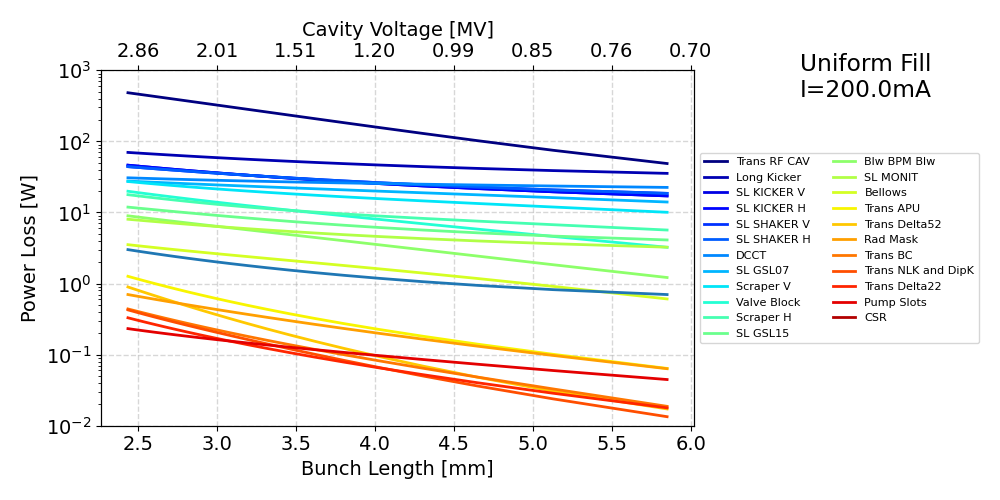
\includegraphics[width=0.48\textwidth]{THPC44_f1.png}
        \caption{Power loss for each component of the impedance budget model as function of the cavity voltage and bunch length.}
        \label{fig:model_vary_vgap}
    \end{figure}
     shows the power loss predicted by the impedance budget model of the SIRIUS storage ring for each component of the vacuum chamber when the gap voltage of the cavity is varied and uniform filling is considered. Note the strong dependence of the power loss with the bunch length. Figure~\ref{fig:model_vary_fillp}
    \begin{figure}
        \centering
        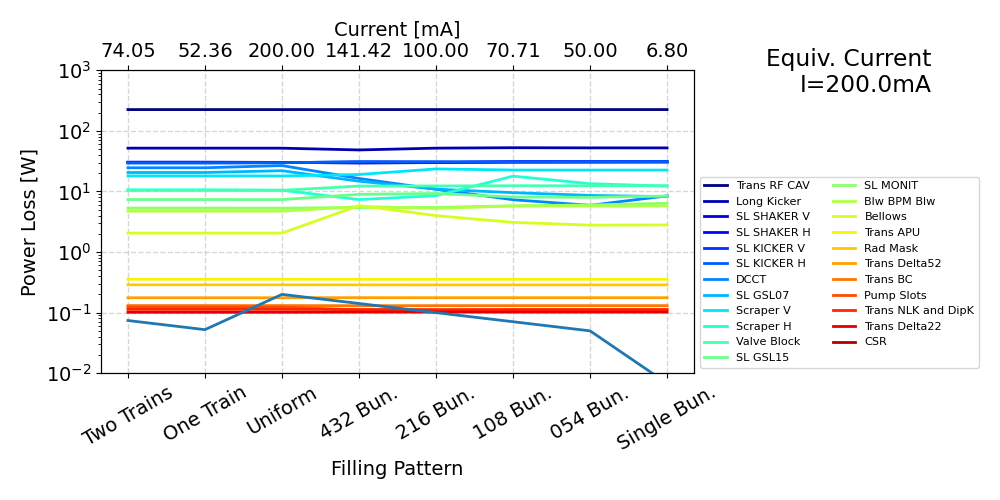
\includegraphics[width=0.48\textwidth]{THPC44_f2.png}
        \caption{Power loss for each component of the impedance budget model for several filling patterns, considering a bunch length of~\SI{3.5}{\milli\meter}. The total current used for each filling pattern was calculated using Eq.~\eqref{eq:power_broadband} so that the equivalent current in uniform filling was kept constant and equal to~\SI{200}{\milli\ampere}. The nomenclature~"$\!N$ Bun." refers to fillings with~$N$ equally spaced bunches.}
        \label{fig:model_vary_fillp}
    \end{figure}
     shows the model prediction for power loss for different filling patterns, keeping the equivalent total power constant, according to Eq.~\eqref{eq:power_broadband}. Since most components are dominated by broadband impedances, the power losses do not depend too much on the filling pattern.
    
    From these results we see that the taper transition of the superconducting rf cavities is the single component with the largest power loss, reaching approximately~\SI{225}{\watt} at~\SI{200}{\milli\ampere} in uniform filling and~\SI{1.6}{\mega\volt} in the rf cavities. Since this component is not installed yet, it will not be possible to check future heating problems. However, this power load was considered in thermal simulations of this component. The second class of components with large power deposition are the striplines (SL), ranging from~\SIrange{20}{50}{\watt} of deposited power, followed by the DCCTs and the vertical scraper.

\section{Experimental results}

    Two machine studies were conducted to probe two approaches of estimation of heat-load. The method of decreasing the cavity voltage was tested first. In practice, the lower cavity voltage reduced the synchrotron tune, decreasing the longitudinal coupled-bunch instability threshold induced by the cavity \glspl{hom}. With the lower tune, the instability was stronger than what is controllable by the~\gls{bbb}. We started with a low gap voltage of~\SI{\sim0.9}{\mega\volt} and increased the current from zero. At~\SI{64}{\milli\ampere} the beam instability started to compromise the low level RF control and we had to increase the voltage. We followed this strategy along the rest of the experiment and reached~\SI{150}{\milli\ampere} with a gap voltage of~\SI{1.35}{\mega\volt} and using~\SI{120}{\kilo\watt} of power. During this study no temperature rise was noted in any sector of the storage ring.
    
    The study with non-uniform fillings started with a single train of filled buckets, as shown in Fig.~\ref{fig:2023-08-01_onetrain_fill}.
    \begin{figure}
        \centering
        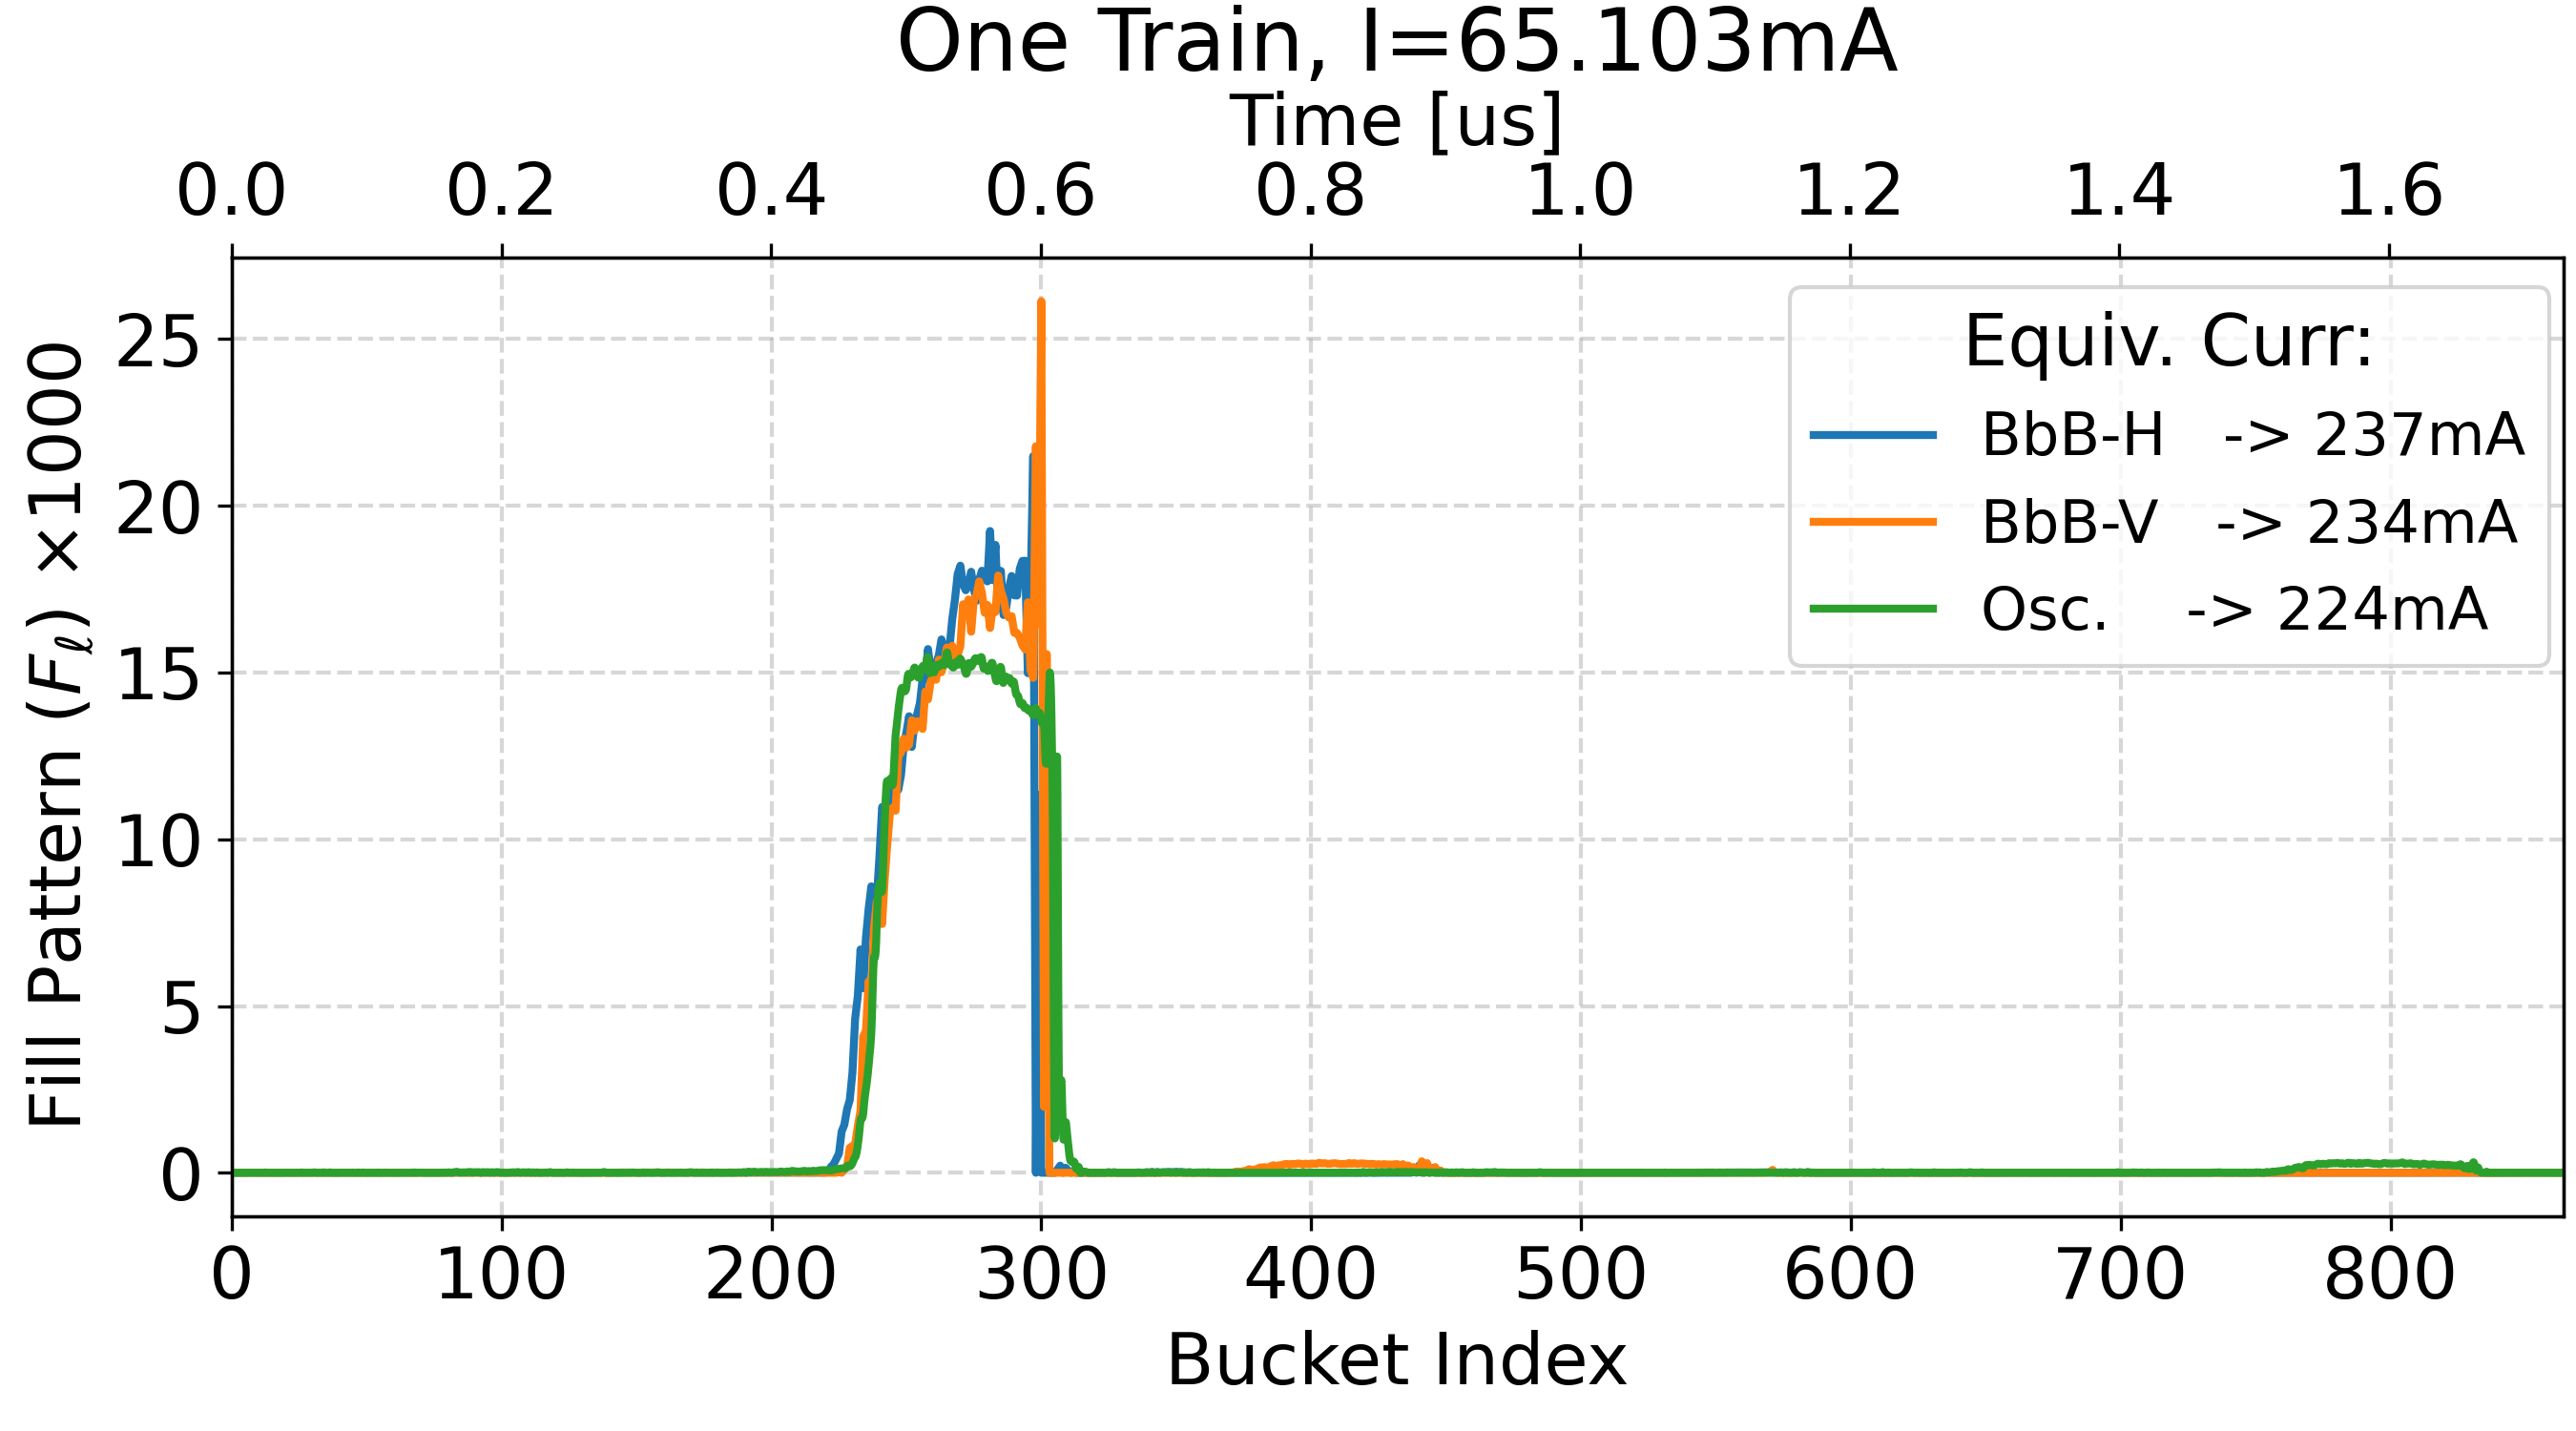
\includegraphics[width=0.95\columnwidth]{THPC44_f3.png}
        \caption{Measurement of filling pattern with three different systems: the vertical and horizontal~\gls{bbb} and a filling pattern oscilloscope. The equivalent current in uniform fill to create the same power deposition was calculated with Eq.~\eqref{eq:power_broadband}.}
        \label{fig:2023-08-01_onetrain_fill}
    \end{figure}
    In this run,~\SI{65}{\milli\ampere} was reached with a single train in the machine. The current could not be increased any further because the temperature of the cavity window was too close from its interlock threshold of~\SI{100}{\celsius}. This high temperature was being induced by coupled-bunch oscillations of the beam, due to \glspl{hom} of the cavity. The current was kept constant in top-up mode for some time to analyse the evolution of the pressure and temperature of the components. No pressure related problems were observed, but one temperature from sector~\num{1} increased and did not stabilize during the whole experiment, reaching~\SI{\approx53}{\celsius} before the beam was dumped, see Fig.~\ref{fig:temps_sector1}.
        \begin{figure}
        \centering
        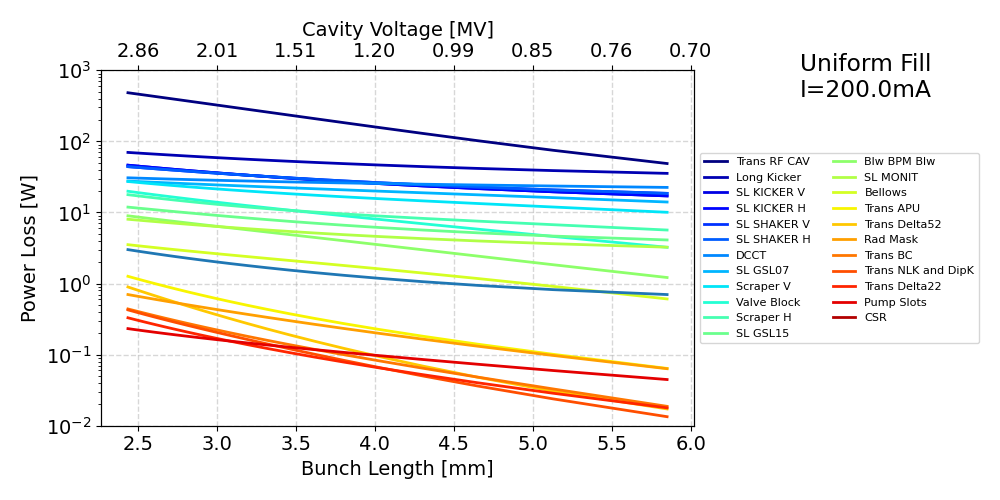
\includegraphics[width=0.95\columnwidth]{THPC44_f4.png}
        \caption{Temperature readouts of the storage ring injection sector during the experiments with non-uniform filling.}
        \label{fig:temps_sector1}
    \end{figure}
    % Unfortunately, it was not possible to identify which component was the source of the observed heating.

    Next, the beam was injected in two trains. Figure~\ref{fig:2023-08-01_twotrains_fill}
    \begin{figure}
        \centering
        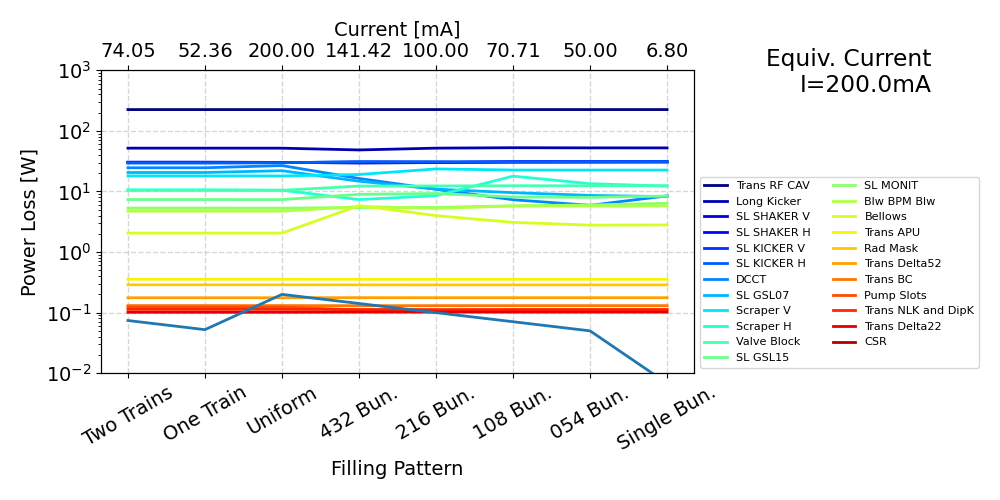
\includegraphics[width=0.95\columnwidth]{THPC44_f5.png}
        \caption{Filling patter measurement, see legend of~Fig.~\ref{fig:2023-08-01_onetrain_fill}.}
        \label{fig:2023-08-01_twotrains_fill}
    \end{figure}
    shows the equivalent current of this filling pattern. In this configuration, it was possible to reach~\SI{90}{\milli\ampere}, keeping the temperature of the cavity window at~\SI{96}{\celsius}. The same heating problem was observed in sector 1. Figure~\ref{fig:temps_sector1} shows the similarity between the heating of the single train experiment with the one with two trains. Both experiments had similar equivalent currents, as shown in Figs.~\ref{fig:2023-08-01_onetrain_fill} and~\ref{fig:2023-08-01_twotrains_fill}. These observations corroborate with the hypothesis of broadband induced power on the component close to the sensor.

    The sensor that showed temperature rise was on a bellows of the injection sector of the machine. However, since this bellows was close to the vertical scraper and there was no other sensor between them, the question remained of which component was indeed heating. For this reason, more temperature sensors were added in the region and a third machine study was carried out, more than~\num{9}~months apart from the first two, to verify which component was heating. Similarly to the previous studies, the configuration of two trains with a total current of~\SI{90}{\milli\ampere} was achieved, resulting in similar heating profile. This time, this condition was kept long enough so that the temperature stabilized around~\SI{50}{\celsius}. The extra sensors helped confirming that indeed was the bellows the component that was heating.
    
    There are other three bellows in the injection straight identical to this one. They are unique in the machine, because their cross-section is elliptical, due to the different shape of the vacuum chamber of that sector. Since only one of them heated, it must be result of some mechanical conformation of this component. On the other hand, there are hundreds of round bellows in the machine and none of them showed any temperature rise. This is an statistical evidence that the broadband impedance of the elliptic-type bellows is more sensitive to mechanic variations. Finally, the level of temperature reached in the experiment will not pose a problem for future operations, confirming that it is very likely that SIRIUS can be operated with at least~\SI{200}{\milli\ampere} without a~\gls{3hc}.

\section{Conclusion}

This study aimed to assess the heating load of operations at higher currents with different proxies. The method based on different filling patterns has shown to be more efficient for such verification in the case of SIRIUS, because it conserves the bunch length. In this context, it was verified experimentally that SIRIUS will probably be able to operate at~\SI{200}{\milli\ampere} without the need of the~\gls{3hc}. It was not possible to test higher currents because of the temperature limitation imposed by the RF cavity window.
%
% only for "biblatex"
%
\ifboolexpr{bool{jacowbiblatex}}%
{\printbibliography}%
{%
% "biblatex" is not used, go the "manual" way

%\begin{thebibliography}{99}   % Use for  10-99  references
    \begin{thebibliography}{9} % Use for 1-9 references

        %\cite{Chao:1993zn}
        \bibitem{Chao:1993zn}
        A.~W.~Chao,
        \textit{Physics of collective beam instabilities in high-energy accelerators},
        John Wiley \& Sons, 1993. \\ \\
        
        \bibitem{Wikipedia_DFT}
        Wikipedia contributors,
        "Discrete Fourier transform --~ Wikipedia, The Free Encyclopedia",\\
        \url{https://en.wikipedia.org/w/index.php?title=Discrete_Fourier_transform&oldid=1153873152}
    \end{thebibliography}
} % end \ifboolexpr


\end{document}
